\documentclass{beamer}
\usepackage[utf8]{inputenc}
\usepackage{helvet}
\usepackage{caption}
\usepackage{xcolor}

\renewcommand{\familydefault}{\sfdefault}

% Define colors
\definecolor{MoneyGreen}{RGB}{0, 166, 126} % Define MoneyGreen
\definecolor{myBulletColor}{RGB}{0, 166, 126} % For bullets
\definecolor{myHeaderColor}{RGB}{0, 166, 126} % For headers

% Apply the colors to the bullets
\setbeamercolor{itemize item}{fg=myBulletColor}
\setbeamercolor{itemize subitem}{fg=myBulletColor}
\setbeamercolor{itemize subsubitem}{fg=myBulletColor}
\setbeamercolor{author in head/foot}{bg=MoneyGreen, fg=white}
\setbeamercolor{title in head/foot}{bg=MoneyGreen, fg=white}
\setbeamercolor{title}{fg=MoneyGreen}
\setbeamercolor{section in toc}{fg=black}
\setbeamercolor{frametitle}{fg=myHeaderColor}

% Footline settings
\setbeamertemplate{footline}{%
  \leavevmode%
  \hbox{%
  \begin{beamercolorbox}[wd=\paperwidth,ht=2.25ex,dp=1ex]{author in head/foot}%
    \usebeamerfont{author in head/foot}%
    \makebox[.3333\paperwidth][l]{\hspace{0.3cm}\myclass\hskip.5cm}%
    \makebox[.3333\paperwidth][c]{\shorttitle}%
    \makebox[.3333\paperwidth][r]{\hskip.5cm\insertframenumber/\inserttotalframenumber\hspace{0.3cm}}%
  \end{beamercolorbox}}%
  \vskip0pt%
}

\newcommand{\myclass}{Digital Tools HS23}
\newcommand{\shorttitle}{Deposit Rate Sensitivity}

% Table of Contents Settings
\setbeamertemplate{section in toc}{\inserttocsectionnumber.~\inserttocsection}
\setbeamertemplate{subsection in toc}{
  \leavevmode\leftskip=4em
  \rlap{\hskip-2em\inserttocsectionnumber.\inserttocsubsectionnumber}
  {\small\inserttocsubsection}\par
}

% Descriptive info
\title{Analysis of Deposit Rate Pass Through Effects in Tightening Cycles}
\institute{University of Zurich}
\author{John Hojnacki, Matthew Alyward, Victoria Gemperle}

% Main content

\begin{document}

\begin{frame}
\titlepage % This will create a title slide with your title, author, and institution
\end{frame}

\begin{frame}
\frametitle{Table of Contents}
\tableofcontents
\end{frame}

\section{Introduction}
\subsection{Motivation}
\begin{frame}
\frametitle{Introduction to Project: Motivation}
\begin{itemize}
  \item When central banks raise policy rates, it's expected that other rates follow suit.
  \item Deposit rates on savings for private consumers are of particular importance because they affect most (98.6 percent) <insert source> households.
  \item How quickly and how much deposit rates "catch up" with policy rates has important implications yet remains difficult to measure due to major differences in starting points for rate hikes over time.
  \item Comparing relative and absolute changes in interest rates alone may result in extreme results that lack meaning, for example an increase of 50 basis points from a starting point of zero or negative rates has no economic interpretation.
\end{itemize}
\end{frame}

\subsection{Approach}
\begin{frame}
\frametitle{Introduction to Project: Approach}
\begin{itemize}
  \item Our project uses a novel approach to compare the response speed and extent of deposit rate sensitivity to policy rate hikes within a country.
  \item We utilize the concept of 'cumulative deposit beta' to measure the total change in deposit rates against policy rates, inspired by recent NY Fed research. <insert reference>
  \item This beta provides a comparative metric across different rate hike cycles.
  \item Our research contributes to the literature by analyzing deposit rate sensitivity in Switzerland and offers an open-source methodology for wider application.
\end{itemize}
\end{frame}

\section{Data and Methodology}
\subsection{Data Requirements}
\begin{frame}
\frametitle{Data and Methodology: Data Requirements}
\begin{itemize}
  \item In principle, only two data sets are needed to run the analysis, policy rates and deposit rates over time.
  \item If one or both of these data sets is unavailable for a sufficient time period, they can be approximated from alternative data with similar economic meaning.
  \item In the NY Fed research that we used for inspiration, deposit rates are estimated using bank financial statements, taking total interest paid over total interest bearing deposits. 
  \item In our own analysis which follows in this presentation, we estimate a policy rate for Switzerland that is the midpoint of an upper and lower target range.
  \end{itemize}
\end{frame}

\subsection{Identification of Hiking Cycles}
\begin{frame}
\frametitle{Data and Methodology: Identification of Hiking Cycles}
The identification of hiking periods is conducted through a systematic algorithm:
\begin{itemize}
  \item Time \( t \) is measured in months.
  \item A hiking period is defined as a sequence of months with an increase in the policy rate.
  \item The algorithm marks a month as 'hiking' if:
  \begin{itemize}
    \item There's an increase in the policy rate from the previous month.
    \item An increase is anticipated in the subsequent two months.
  \end{itemize}
  \item Months preceding a rate hike are also included in the hiking period.
  \item Unique identifiers are assigned to each hiking period for analysis.
\end{itemize}
\end{frame}

\subsection{Calculation of Deposit Betas}
\begin{frame}
\frametitle{Data and Methodology: Calculation of Deposit Betas}
We estimate the deposit beta (\( \beta_t \)) to measure how deposit rates respond to policy rate changes:
\begin{equation}
\beta_t = \frac{\Delta D_t}{\Delta P_t}
\end{equation}
where:
\begin{itemize}
  \item \( \Delta D_t \) is the total change in the deposit rate,
  \item \( \Delta P_t \) is the total change in the policy rate,
  \item \( t \) denotes time in months from the start of the hiking cycle.
\end{itemize}
A higher \( \beta_t \) indicates a stronger response of deposit rates to policy changes. We track \( \beta_t \) evolution from the cycle's onset to the peak of deposit rates.
\end{frame}

\section{Swiss Case Study}
\subsection{Applying the Methodology}
\begin{frame}
\frametitle{Swiss Case Study: Applying the Methodology}
\textbf{Research Question:}
\begin{itemize}
  \item How does the most recent hiking cycle compare to past cycles in Switzerland?
\end{itemize}
\textbf{Data:}
\begin{itemize}
  \item To answer the research question, we use publicly available data from the Swiss National Bank data portal.
  \item Switzerland had a target policy range from 2000-2019, here we use the midpoint. From 2019 onwards, we use the actual target value.
  \item Deposit rates for private customers are provided in monthly format and are utilized directly.
\end{itemize}
\end{frame}

\subsection{Interest Rates over Time}
\begin{frame}
\frametitle{Swiss Case Study: Interest Rates over Time}
\text{Historical visualization of interest rates in Switzerland}
\begin{center}
\begin{minipage}{0.8\textwidth}
\begin{figure}[H]
    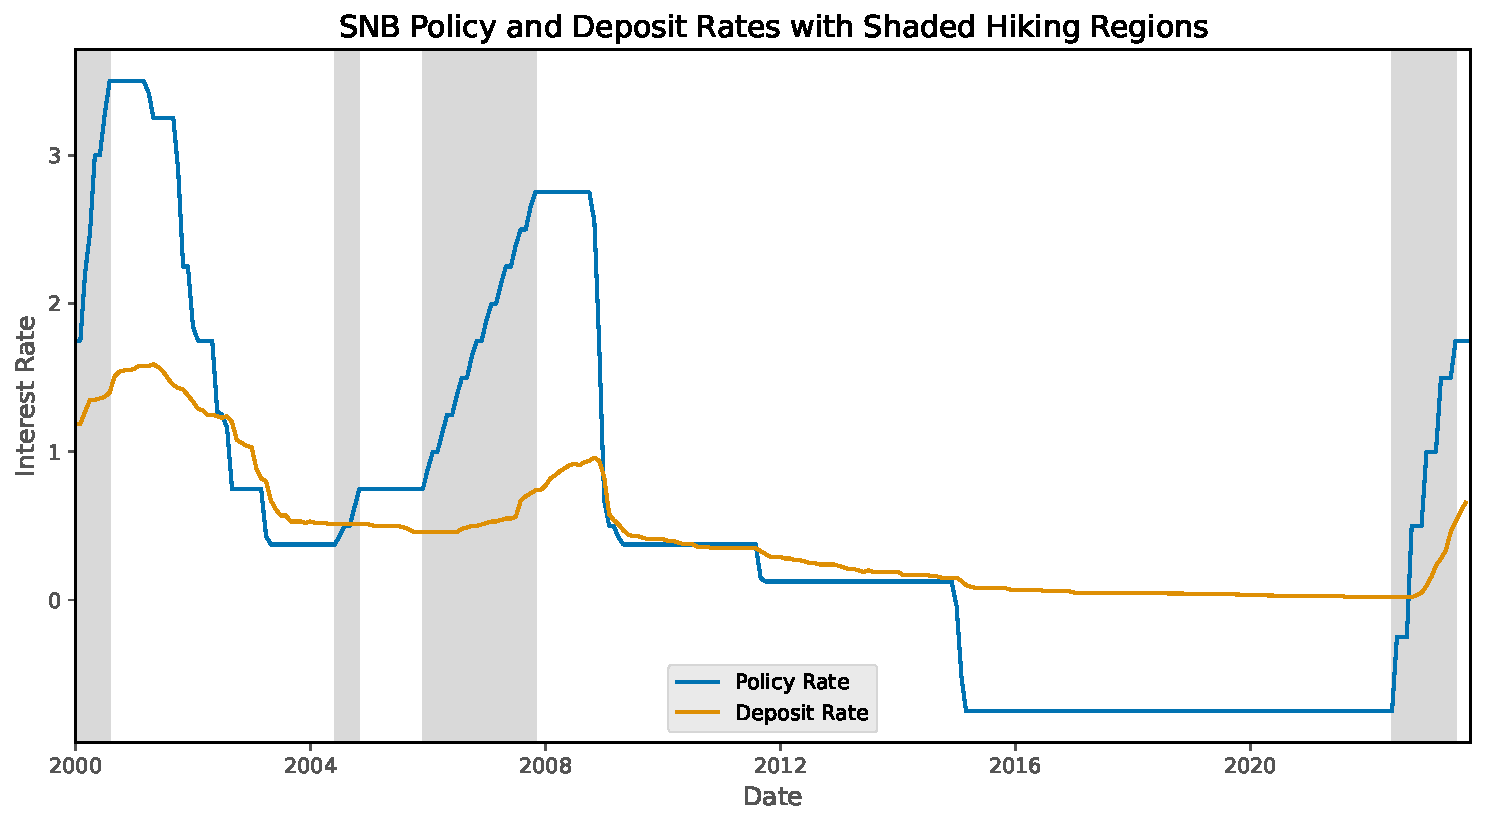
\includegraphics[width=\textwidth]{Test/rates_shaded_SNB.pdf}
    \captionsetup{font=tiny,labelfont={color=black},justification=raggedright,singlelinecheck=off}
    \caption{Policy and Deposit Rates for Switzerland}
    \label{fig:rates_shaded}
\end{figure}
\end{minipage}
\end{center}
\end{frame}

\subsection{Hiking Cycle Identification}
\begin{frame}
\frametitle{Swiss Case Study: Hiking Cycle Identification}
\text{Identification of Hiking Cycles and Rising Deposit Rates}

\begin{center}
\begin{minipage}{0.8\textwidth}
\begin{figure}[H]
    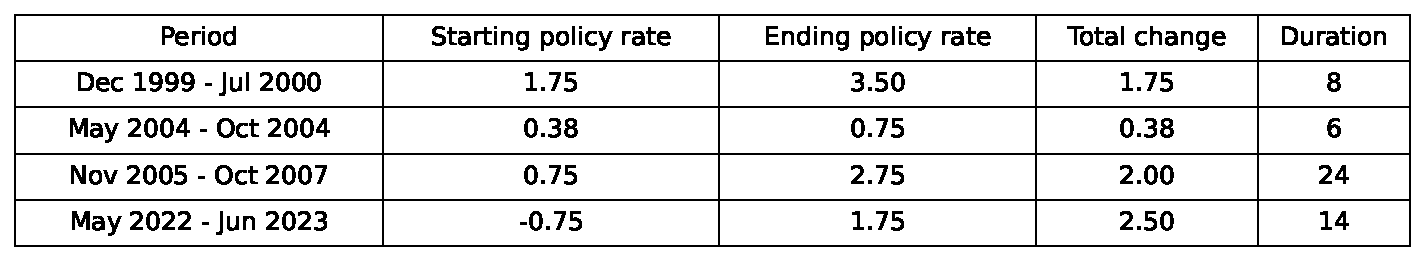
\includegraphics[width=\textwidth]{Test/hiking_summary_SNB.pdf}
    \captionsetup{font=tiny,labelfont={color=black},justification=raggedright,singlelinecheck=off}
    \caption{Hiking Cycles Across Time}
    \label{fig:hiking_summary}
\end{figure}
\end{minipage}
\end{center}

\begin{center}
\begin{minipage}{0.8\textwidth}
\begin{figure}[H]
    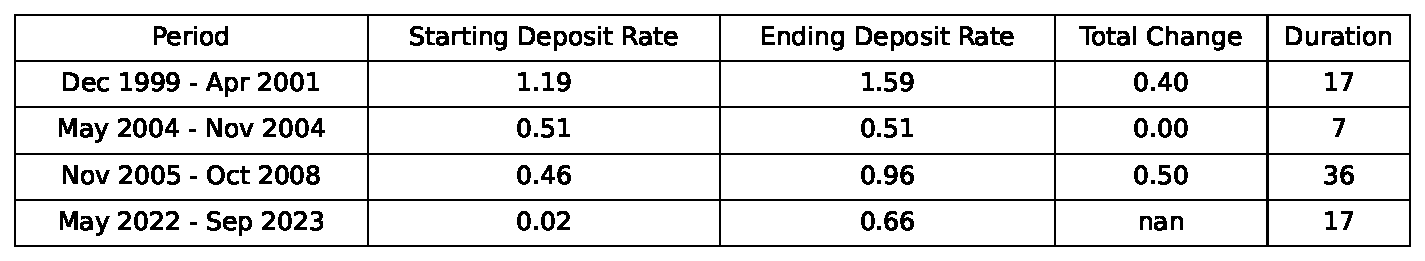
\includegraphics[width=\textwidth]{Test/deposit_summary_SNB.pdf}
    \captionsetup{font=tiny,labelfont={color=black},justification=raggedright,singlelinecheck=off}
    \caption{Deposit Rates Summary across Hiking Periods}
    \label{fig:deposit_summary}
\end{figure}
\end{minipage}
\end{center}
\end{frame}

\subsection{Deposit Betas}
\begin{frame}
\frametitle{Swiss Case Study: Deposit Betas}
\text{Charting Deposit Betas over Time}
\begin{center}
\begin{minipage}{0.8\textwidth}
\begin{figure}[H]
    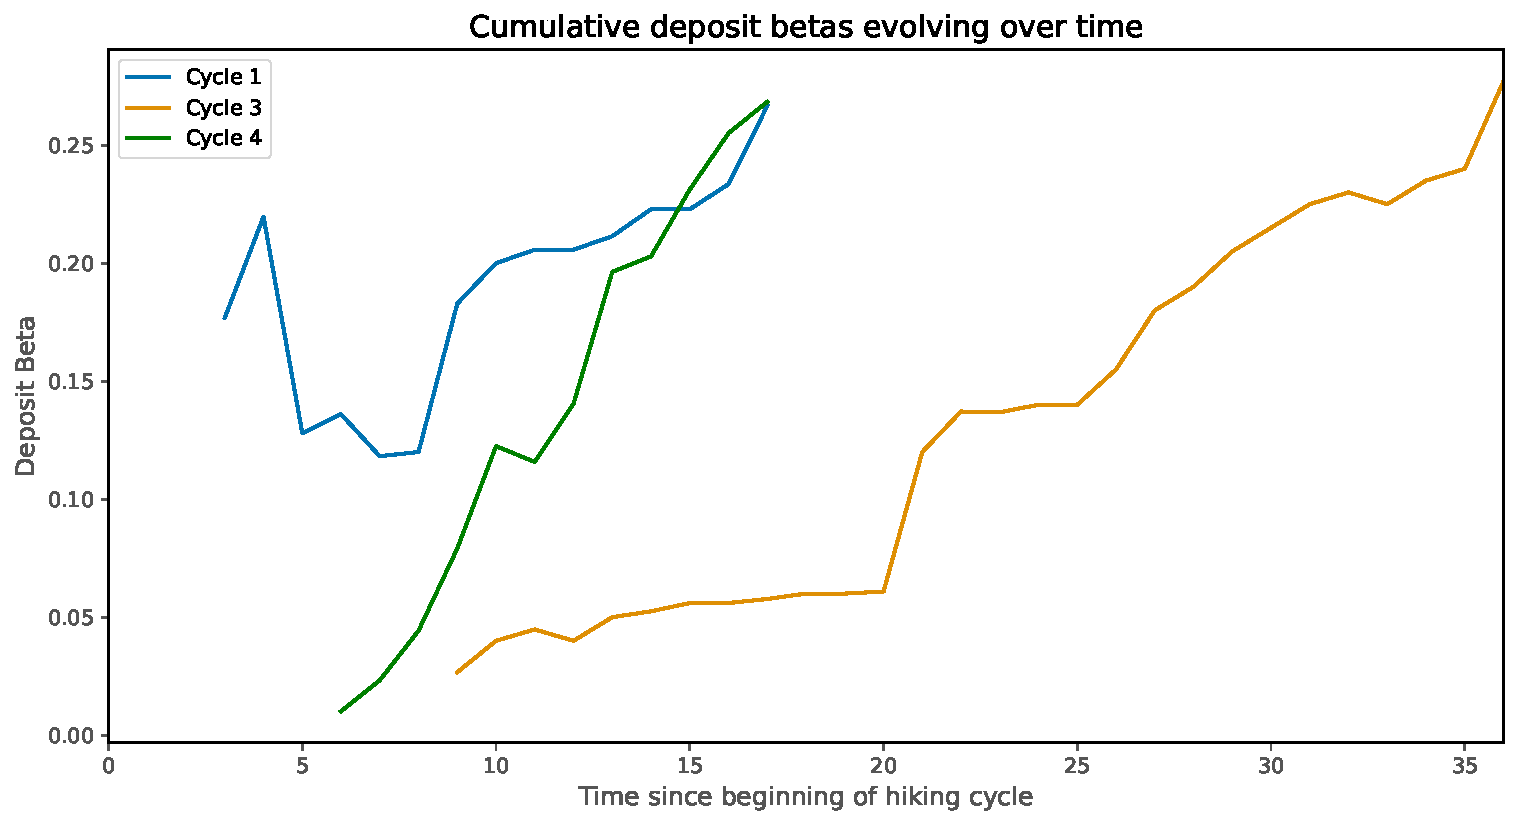
\includegraphics[width=\textwidth]{Test/deposit_beta_SNB.pdf}
    \captionsetup{font=tiny,labelfont={color=black},justification=raggedright,singlelinecheck=off}
    \caption{Deposit Rates Summary across Hiking Periods}
    \label{fig:deposit_summary}
\end{figure}
\end{minipage}
\end{center}
\end{frame}

\subsection{Analysis of Results}
\begin{frame}
\frametitle{Swiss Case Study: Analysis of Results}
\begin{itemize}
    \item bullet 1
    \item bullet 2
    \item bullet 3
\end{itemize}
    
\end{frame}

\section{Project Architecture}
\begin{frame}
\frametitle{Project Architecture}
\textbf{Research Question:}
\begin{itemize}
  \item cloud cloud cloud cloud cloud cloud cloud cloud cloud cloud cloud cloud cloud cloud cloud cloud cloud cloud
\end{itemize}

\textbf{Our Approach:}
\begin{itemize}
  \item cloud cloud cloud cloud cloud cloud cloud cloud cloud cloud cloud cloud cloud cloud cloud cloud cloud cloud cloud cloud cloud cloud cloud cloud cloud cloud cloud cloud cloud cloud cloud cloud cloud cloud cloud cloud
\end{itemize}
\end{frame}

\begin{frame}
\frametitle{Project Architecture (cont...)}
\textbf{Research Question:}
\begin{itemize}
  \item cloud cloud cloud cloud cloud cloud cloud cloud cloud cloud cloud cloud cloud cloud cloud cloud cloud cloud
\end{itemize}

\textbf{Our Approach:}
\begin{itemize}
  \item cloud cloud cloud cloud cloud cloud cloud cloud cloud cloud cloud cloud cloud cloud cloud cloud cloud cloud cloud cloud cloud cloud cloud cloud cloud cloud cloud cloud cloud cloud cloud cloud cloud cloud cloud cloud
\end{itemize}
\end{frame}

\end{document}

